\section{Meta Pattern}
\begin{itemize}
    \item Reflection is often used as technology for Meta Programming
    \item Provide Flexibility, Adaptability \& Generality
\end{itemize}
\textbf{Recurring Problems}
\begin{itemize}
    \item Reflection solves common frameworkers problems
    \item Exchanging parts of a software system is hard
    \item Not yet unknown sofware components should be integrated
\end{itemize}

\subsection{Reflection}
\textbf{Usage (Java / C\#)}
\begin{itemize}
    \item Load of JAR / DLL
    \item Invoke Methods 
    \item Read out properties/fields 
    \item Create object instances 
    \item Search for annotations on Classes / Methods / Fields / ...
\end{itemize}
\textbf{Provides Facility to implement:}
\begin{itemize}
    \item DI
    \item Convention over Configuration
    \item Object-Relation Mapper
    \item Serialization / Deserialization
    \item Plugin Architectures
\end{itemize}
Consists of two aspects:\\ 
\textbf{Introspection}
\begin{itemize}
    \item The ability for a program to observe and therefore reason about its own state
    \item e.g. Query object properties, get list of methods
\end{itemize}
\textbf{Intercession}
\begin{itemize}
    \item The ability of a program to modify its own execution state or alter its own interpretation of meaning
    \item e.g. Modify object properties, add another attribute or exchange code
\end{itemize}
Defines meta level and base level:\\ 
\textbf{Meta level}
\begin{itemize}
    \item Provides self-representation
    \item Gives the SW a knowledge of its own structure
    \item Consists of meta objects
\end{itemize}
\textbf{Base level}
\begin{itemize}
    \item Defines the app logic
    \item Implementation may use the meta objects
\end{itemize}
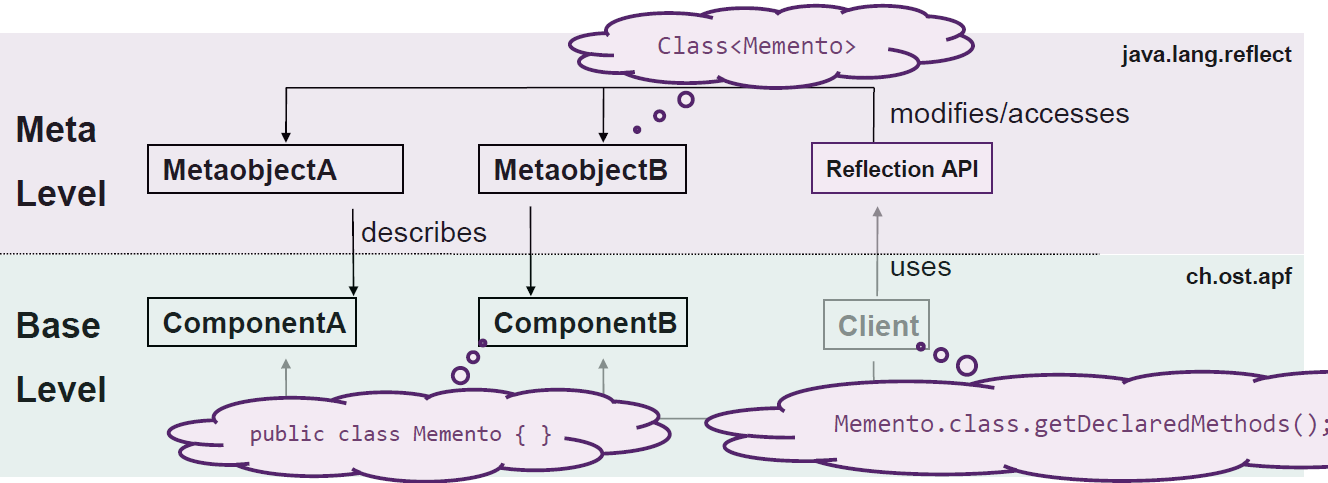
\includegraphics[width=\linewidth]{./img/meta_base_level.png}
\subsubsection{Summary}
\textbf{Benefits}
\begin{itemize}
    \item Adapting a software system is easy
    \item Support for many kinds of changes
\end{itemize}
\textbf{Liabilities}
\begin{itemize}
    \item Produces non-transparent APIs
    \item Binding at runtime (limited Type safety)
\end{itemize}

\subsection{Meta Objects}
\textbf{Usage}
\begin{itemize}
    \item Classes
    \item Object Attributes
    \item Methods
    \item Class Relationships
\end{itemize}

\subsection{Type Object}
\subsubsection{Problem}
\begin{itemize}
    \item We want to keep common behaviour and data in only one place
    \item DRY implementation of domain
    \item How can you categorize objects, eventually dynamically?
\end{itemize}
\subsubsection{Solution}
Categorize objects by another object instead of a class. Thus an object can change it's 'class' at runtime
\begin{itemize}
    \item Create a category (type) object which describes multiple objects
    \item Objects forward the calls to the underlying type
\end{itemize}
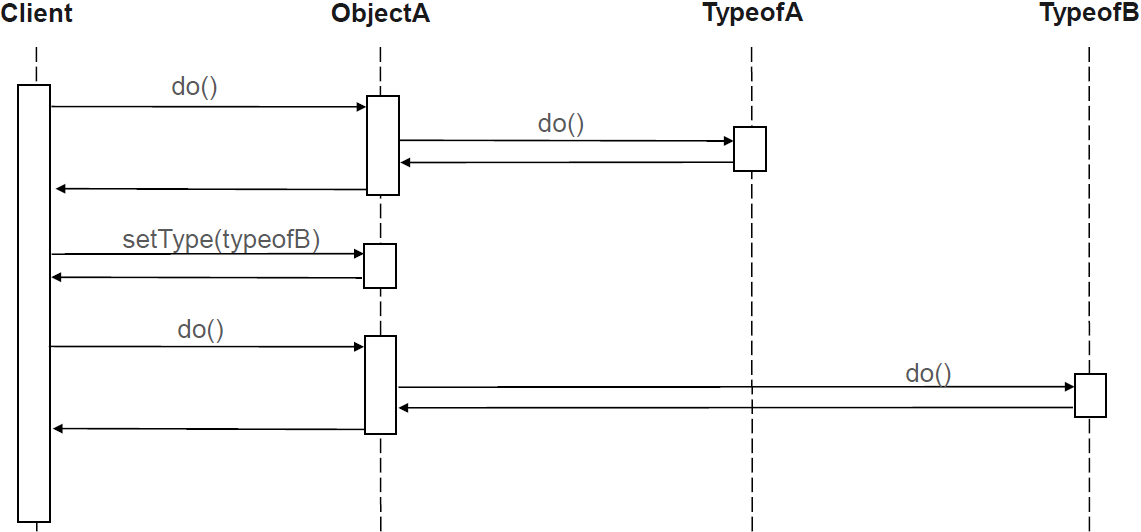
\includegraphics[width=\linewidth]{./img/type_object.png}
\subsubsection{Summary}
\textbf{Benefits}
\begin{itemize}
    \item Categories can be added easily, event at runtime
    \item Allows multiple meta-levels
\end{itemize}
\textbf{Liabilities}
\begin{itemize}
    \item Confusing mess of 'classes' because of separation
    \item Lower efficiency because of indirection
    \item Changing database schemas can be tricky
\end{itemize}
\subsubsection{Discussion}
\textbf{Based on which GoF Pattern}
\begin{itemize}
    \item Strategy
\end{itemize}
\textbf{Similar intent in a GoF Pattern}
\begin{itemize}
    \item State, also changes at runtime
\end{itemize}

\subsection{Property List}
\subsubsection{Problem}
\begin{itemize}
    \item Attributes should be attachable / detachable after compilation
    \item Objects share attributes / parameters across the class hierarchy
    \item How do you define properties in a flexible way so they can be attached and detached at runtime?
\end{itemize}
\subsubsection{Solution}
Provide objects with a property list. That list allows to associate names with other values or objects.
\begin{itemize}
    \item Property list maps attribute names to values
    \item each name defines a slot
    \item Same slot can be used for attributes with identical semantics
    \item Objects can be triggred to list all slot names and values
\end{itemize}
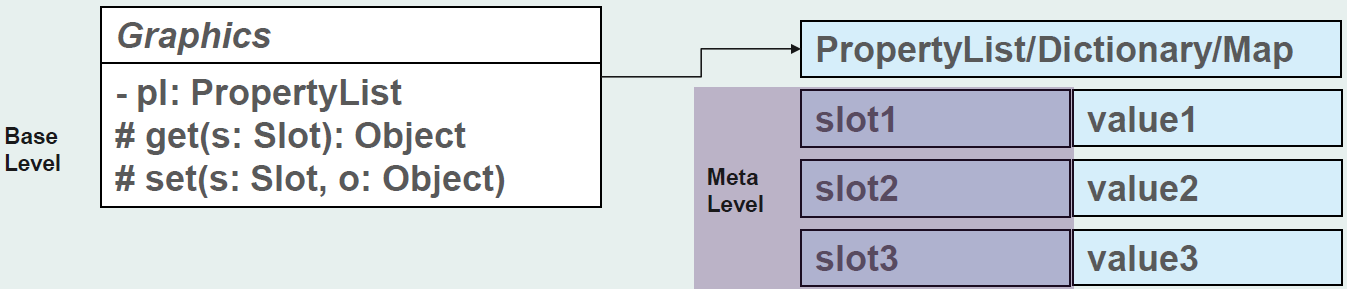
\includegraphics[width=\linewidth]{./img/property_list.png}
\subsubsection{Summary}
\textbf{Benefits}
\begin{itemize}
    \item Attributes can be added dynamically
    \item Object extension while keeping object identity
    \item Easy attribute iteration
\end{itemize}
\textbf{Liabilities}
\begin{itemize}
    \item Different ways to access regular / dynamic attributes
    \item Type safety left to the programmer
    \item Run-time overhead
    \item Memory Management
\end{itemize}
\textbf{Mitigate Liabilities:} Bridge Methods

\subsection{Anything}
\begin{itemize}
    \item Arbitrary data structure
    \item Recursively structured Property List
    \item Internal representation of today's JSON
\end{itemize}
\textbf{Object Definition:}
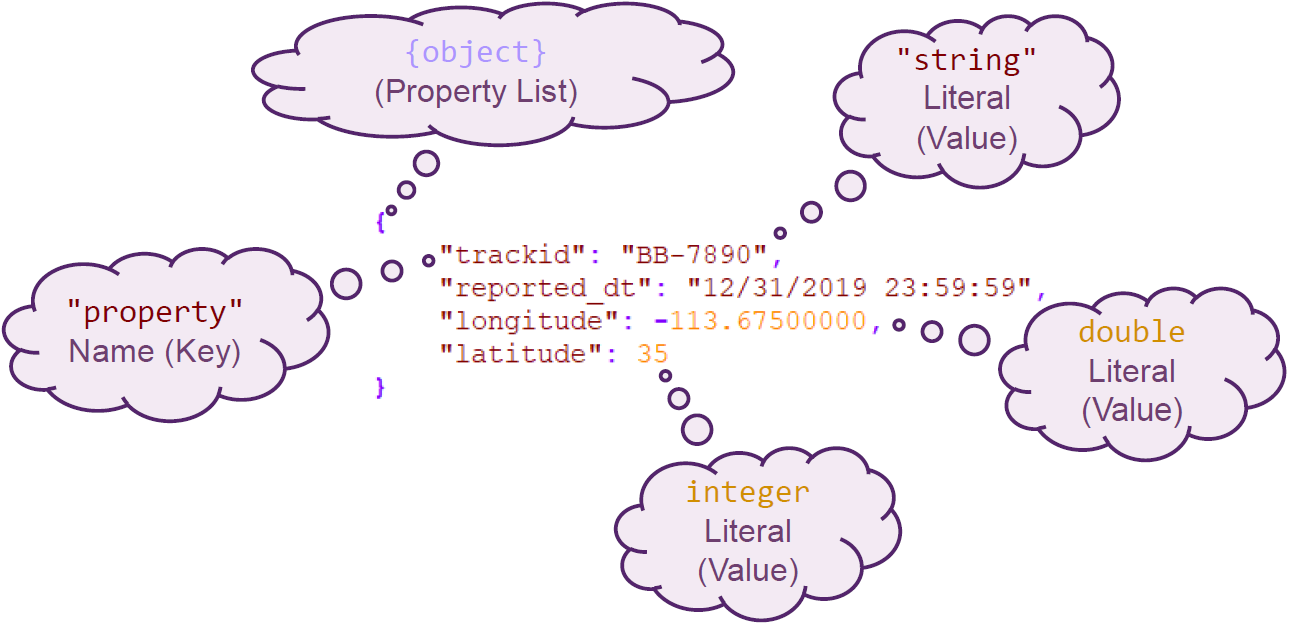
\includegraphics[width=\linewidth]{./img/anything.png}
\subsubsection{Problem}
\begin{itemize}
    \item We need to keep a map of data similar to the Property List
    \item Structured data also includes sequences of data
    \item Data should be structured recursively
    \item How do you provide a generic configuration or communication data structure that is easily extensible?
\end{itemize}
\subsubsection{Solution}
Create an abstraction for structured values that is self describing.
\begin{itemize}
    \item Implement a representation of simple values
    \item Add an implementation for a sequence of values (\& key value access)
    \item Provide a default value
\end{itemize}
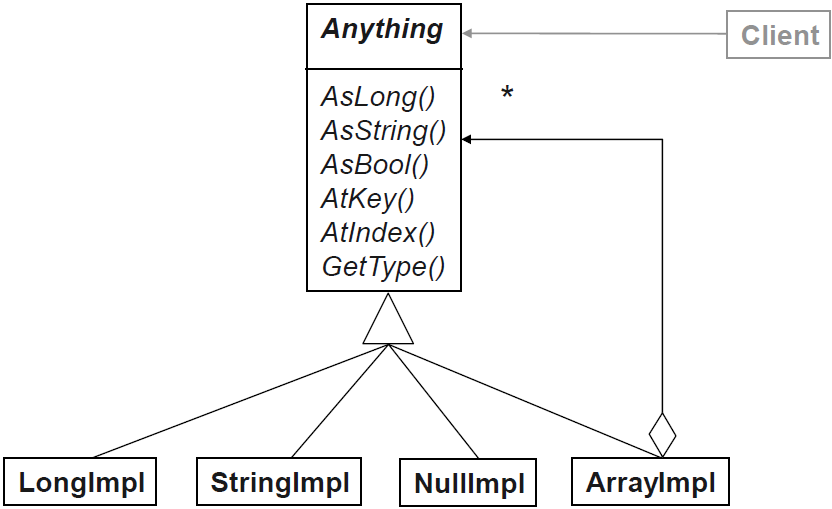
\includegraphics[width=\linewidth]{./img/anything_uml.png}
\subsubsection{Summary}
\textbf{Benefits}
\begin{itemize}
    \item Readable streaming format
    \item Appropriate for configuration data
    \item Universally applicable
    \item Flexible interchange across class/object boundaries
\end{itemize}
\textbf{Liabilities}
\begin{itemize}
    \item Less type safety
    \item Intent of parameter elements not always obvious
    \item Overhead for value lookup and member access
    \item No real object, just data
\end{itemize}
\subsubsection{Discussion}
\textbf{Which GoF Pattern does Anything implement?}
\begin{itemize}
    \item Transparent Composite Pattern
    \item Null Object
\end{itemize}
